\documentclass[../main.tex]{subfiles} 
\begin{document}

\chapter{MATERIALER OG METODE}
I denne seksjonen beskrives alt som ble brukt under utviklingen, og hvilke metoder som ble brukt til å løse hovedproblemstillingene, og for å styre gruppen.
\section{Data}
\subsection{Fronter}
Fronter er en kompleks læringsplattform for bruk på skoler. Den tilbyr en omfattende grunnpakke som elever og lærere kan bruke for å kommunisere og samarbeide om skolearbeid. Dette innebærer funksjoner som beskjeder fra lærere, tilgjengeliggjøring av dokumenter og læringsmateriell, innleveringer og prøver, og chat. Fronter tilbyr også en rekke utvidelsesmoduler for spesielle behov, som enkel bilderedigering, SMS og plagiatkontroll.\newline
Fronter sin salgsmodell er en såkalt SaaS modell. Dette vil si at Fronter selger lisenser for bruk av sin programvare, men at de er vert for sine egne web servere. På denne måten trenger ikke kundene å drifte sine egne servere. Dette gjør fronter til et godt alternativ både for små og store institusjoner da det eneste som kreves av kunden er tilgang til en nettleser for sine brukere.

\subsection{TimeEdit}
Timeplan administrasjonssystemet TimeEdit er et system brukt av store institusjoner for å administrere og allokere lokaler. Tjenesten tillater brukerne å se timeplanen for en person, klasse, studieretning eller lokale for et ønsket tidsintervall. Høgskolen I Ålesund bruker TimeEdit versjon 1.4.8 hvor alle tjenestens data lagres og administreres lokalt på skolens servere.

\subsection{BibSys}
Biblioteksystemet BibSys er et arkiveringssystem for bøker og annen media relatert til driften av norske bibliotek. Systemet tillater brukere å søke etter, låne ut, levere inn og reservere bøker ved alle norske bibliotek tilknyttet systemet. Systemet er underlagt Kunskapsdepartementet, men blir administrert ved NTNU i Trondheim.

\section{Verktøy}
Alle gruppemedlemmene brukte Netbeans som IDE til programmeringen av både Android applikasjonen og Java EE webapplikasjonen. Til utviklingen av Android applikasjonen ble også det offisielle Android SDKet (Software Development Kit) brukt. For å få støtte til Android prosjekter i NetBeans brukte vi tredjeparts pluginen NBAndroid. Glassfish Server Open Source Edition ble brukt som plattform for webapplikasjonen.\newline
\newline
Vi ønsket å bruke LaTeX til å skrive prosjektrapporten, men fant ingen prosjektmal fra skolen. Derfor utviklet vi vår egen mal basert på skolen eksisterende prosjektmaler i andre format. Denne malen ligger offentlig tilgjengelig på GitHub.

\section{Materialer}
\subsection{Smartelefon - Galaxy Nexus}
En av de to enhetene som ble brukt til å teste mobilapplikasjonen under utviklingen var smarttelefonen Galaxy Nexus, produsert av Samsung. Denne modellen går også under modellnavnet GT-I9250. Gruppen hadde 3 slike telefoner til rådighet(en for hvert gruppemedlem). Telefonene kjørte under utviklingen Android versjon 4.2.1, kodenavn Jelly Bean.
\subsection{Tablet - Nexus 7}
Dette nettbrettet er et 7 tommers nettbrett produsert av Asus for Google. Det var helt nytt under produksjonsfasen, og tilbød veldig gode spesifikasjoner til en fornuftig pris. Nettbrettet ble brukt til testing av applikasjonen for andre skjermstørrelser(sammenlignet med Galaxy Nexus), og for demonstrasjon. Nettbrettet kjørte Android versjon 4.2.2 under utviklingen.

\subsection{Server}
Prosjektet fikk tildelt en virtuell Ubuntu linux server på skolens VMWare vSphere cluster. På denne ble glassfish installert og webapplikasjonen publisert.

\begin{figure}[h!]
        \centering
        \begin{subfigure}[b]{7cm}
                \centering
                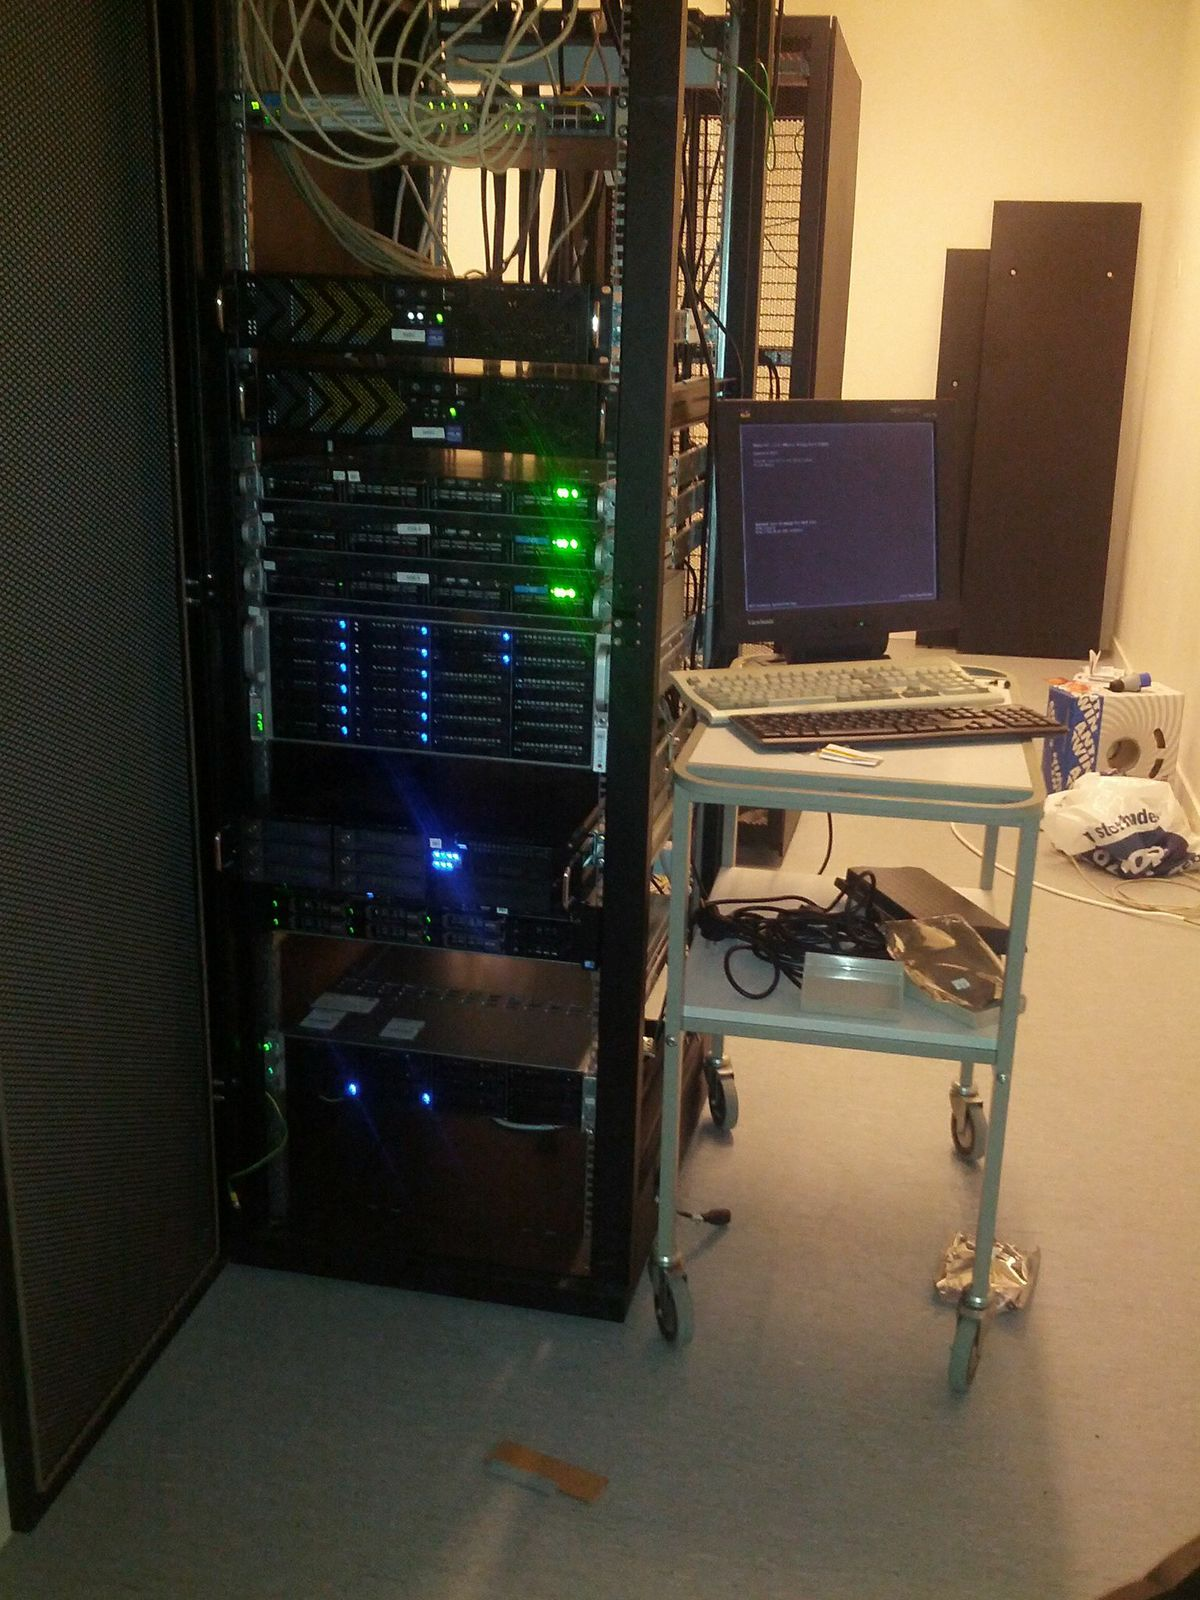
\includegraphics[width=\textwidth]{server1.jpg}

        \end{subfigure}
        \begin{subfigure}[b]{7cm}
                \centering
                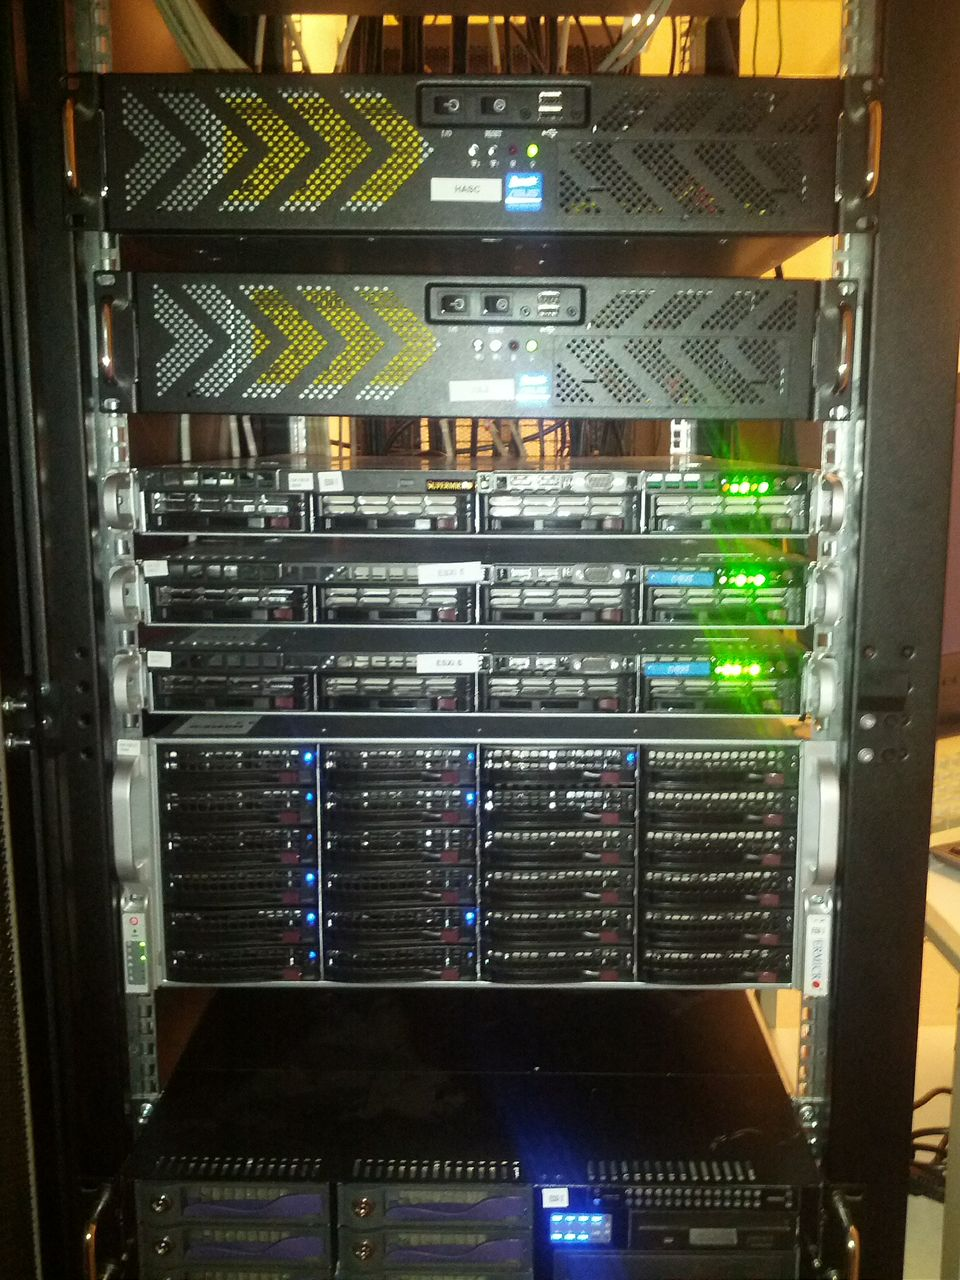
\includegraphics[width=\textwidth]{server2.jpg}

        \end{subfigure}
        \caption{Bilder av serveren}
\end{figure}

\section{Utviklingssyklus}
Under prosjektet tok gruppen utgangspunkt i SCRUM rammeverket, men det ble fort etablert en egentilpasset samarbeidsstil som passet til gruppen. Denne nye stilen innebærte bi-ukentlige statusmøter, daglige statusrapportering blant gruppemedlemmene dog ikke nødvendigvis ved starten av dagen og ikke like formelt som i SCRUM.\newline
\newline
For arbeidet i seg selv ble det brukt to online løsninger som gjorde det mulig å sammarbeide på det samme prosjektet samtidig. For programmeringen var det kildekode-delingstjenesten GitHub som ble brukt. Med denne tjenesten kunne alle gruppemedlemmene sitte med hver sin kopi av arbeidet, og når det ble gjort fremskritt ble dette sendt tilbake til serveren slik at den nye koden blir tilgjengelig for alle. \newline
For prosjektrapporten ble det brukt tekstbehandleren Google Docs. Denne gjør at alle gruppens medlemmer kan jobbe med det samme dokumentet samtidig, og se hva de andre skriver i sanntid. I tillegg har Google Docs innebygd chat funksjon og mulighet til å legge igjen kommentarer i teksten. Grunnen til at disse to tjenestene ble valgt var at alle gruppens medlemmer har god erfaring med dem, og at de tillater en stor grad av sammarbeid uavhengig om deltakerne fysisk befinner seg på samme sted. I sluttfasen av prosjektrapport ble teksten fra Google Docs gjort om til LaTeX format for å kunne bedre kontrollere utseende til den endelige rapporten.

\section{Framgangsmetode}
Denne delen av rapporten omhandler prosjektgruppens framgangsmetode for å løse hovedproblemstillingene.

\subsection{Fronter}
Fronter er et lukket system og derfor måtte vi ha tilgang til APIet for å hente informasjon fra det. Informasjonen vi ønsket å hente var meldinger fra læreren, dokumenter og innleveringsstatus fra de individuelle rommene i Fronter-systemet. For å løse dette skulle mobilapplikasjonen gjøre relevante foresprsler mot en REST basert API på webapplikasjonen. Webapplikasjonen skulle så hente ut relevante data fra Fronter, og returnere det til mobilapplikasjonen, hvor de blir presentert til brukeren.
\subsection{TimeEdit}
Vi ønsket å implementere en enkel utgave av skolens timeplansystem i e-læringsapplikasjonen. Det skulle være mulig å se dagens fag på en enkel måte. Planen var å skaffe tilgang til TimeEdit sitt API, og innhente data derifra via serveren vår ved hjelp av enkle spørringer basert på REST og JSON. Mobilapplikasjonen skulle altså kunne gjøre et kall mot serveren hvor den ba om informasjon om dagens timer/fag for et studieprogram, og så skulle serveren gjøre kallet videre til TimeEdit.
\subsection{BIBSys}
Det kom tidlig frem at BiBSys hadde et API som var tilgjengelig til bruk for studenter og andre utviklere. Dette kunne man se fra antall student-utviklede applikasjoner ved NTNU. Utifra dette ville vi forsøke å få tilgang til APIen og implementere det i webapplikasjonen. Vi ønsket å implementere boksøk med utlånsstatus. Dette var en del av prosjektet vi forventet ville gå relativt raskt og uten problemer.

\subsection{Videreutvikling av applikasjonene}
I den forrige versjonen av systemet var strukturen hardkodet inn i mobilapplikasjonen. Vi ønsket å gjøre systemet mer fleksibelt slik at det kunne tilpasses de individuelle fagene og studienes behov for data. Vi ville at strukturen på mobilapplikasjonen skulle defineres for hvert objekt i webapplikasjonen.

\subsection{Arbeidsprosessen}
Arbeidet i prosjektet skulle i utgangspunktet (ved prosjektstart) være styrt av aktivitetsplanen samt prosedyrer for avvik som ble definert i forprosjektsrapporten. Diagrammet som følger beskriver den faktiske tidsfordelingen mellom de forskjellige delprosjektene.
\begin{figure}[H]
  \centering
  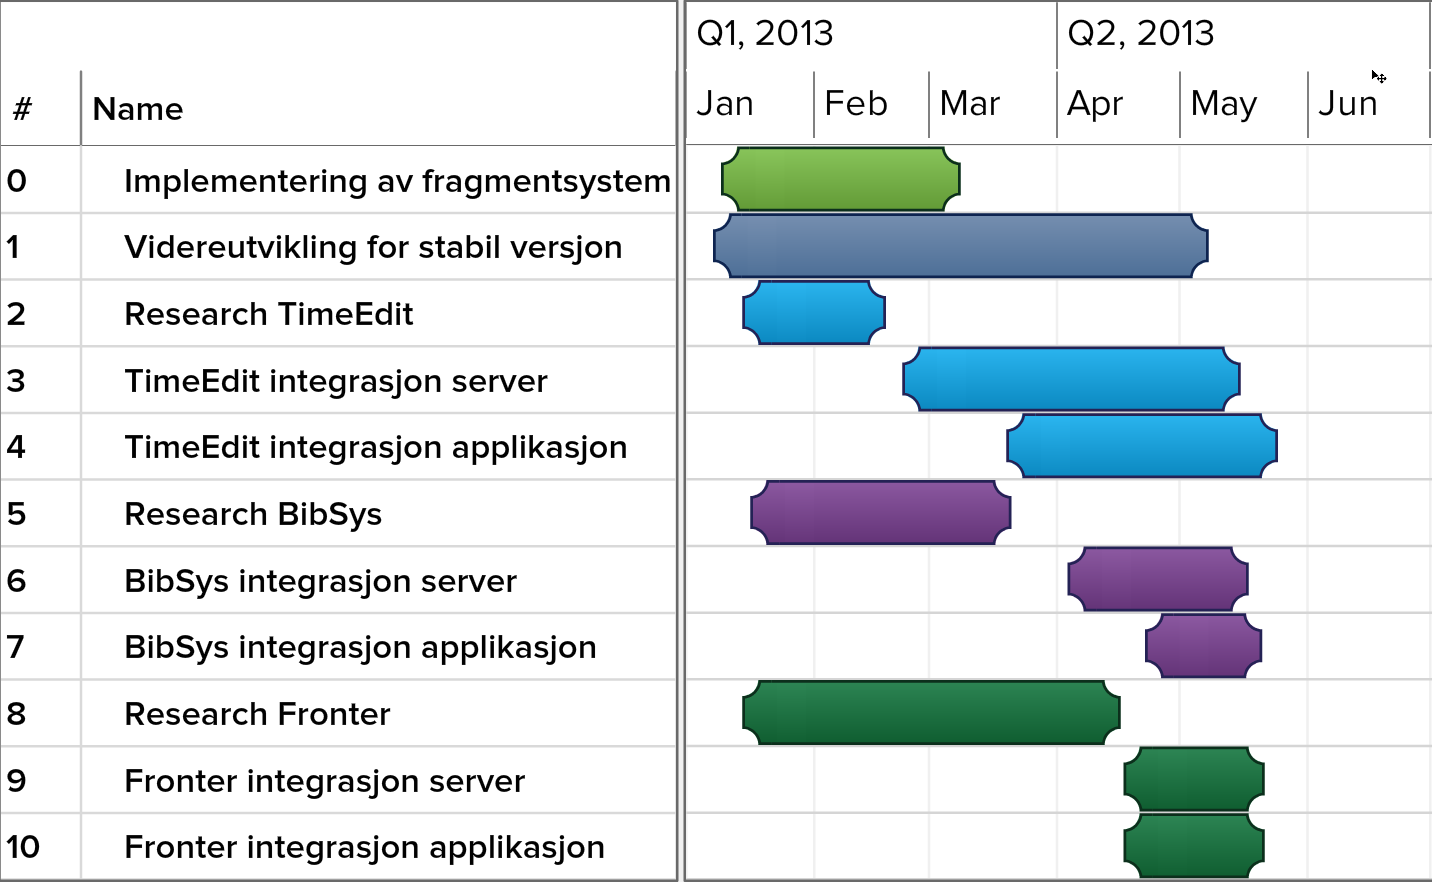
\includegraphics[width=9cm]{Gantt.png}
  \caption{Dette Gantt diagrammet viser når de forskjellige deloppgavene i prosjektet ble utført}
\end{figure}
Ved prosjektstart under den initielle planleggingsfasen (ref. Forprosjektsrapport) ble det klart at å først utvikle en stabil versjon av systemet var nødvendig, og dermed ble arbeid med både web-applikasjon og mobil-applikasjon prioritert først. Under videreutviklingen av systemet ble også ett sett med nye funksjoner inkludert, b.la et fragmentsystem (beskrevet i kap.<dfdsfsdffs<dsfsdfdsfs) felles for mobil og web-applikasjon, samt nytt design for web-applikasjonens nettleser-grensesnitt. Det meste av arbeidet gjort her går likevel under stabilisering av applikasjonene ved å rette bugs og utbedre logisk flyt i systemet. \newline
Parallelt med dette startet vi også å undersøke tilgangsforholdene rundt de forskjellige tjenestene (TimeEdit, BibSys, Fronter) som vi skulle integrere i applikasjonen. Korrespondanse med leverandørene og eierene av datasystemene for å få tilgang til systemenes API tok lengre tid enn forventet, og det ble relativt tidlig (ca. uke 3) klart at vi måtte gå vekk fra den originale tidsplanen.\newline
Målsetningen med å ha utført prosessene A1-B2 går likevel i orden da innsamling av data så langt det var mulig og planlegging av arbeid videre ble gjort innenfor satt tidsfrist. TimeEdit blir prioritert under denne fasen da vi kunne starte forarbeidet umiddelbart med å forsøke alternative løsninger for innhenting av data, noe som også var innenfor det vi hadde forventet (ref. avvik forprosjektsraport). Milepæl \#1 nås imidlertid ikke da undersøkings-delen (pkt.2 i figur \#\#) tok lengre tid enn forventet, og fra dette punktet av omorganiseres prosjektets framdriftsplan helt.\newline
Den nye prosjektorganiseringen var vellykket da det var tid som var den begrensende ressursen, og ikke arbeidskraft.

\newpage

\end{document}